\documentclass[a4paper,11pt,titlepage,uplatex]{jsarticle}

% プリアンブルを外部ファイル化しておきました。中身はmacro.texで確認できます。

\usepackage[dvipdfmx]{graphicx,xcolor}% ドライバ指定
\usepackage[top=30truemm,bottom=30truemm,left=25truemm,right=25truemm]{geometry} % 余白設定

% 画像
\usepackage{here, subfig}
\usepackage{docmute} % ファイル分割用
\usepackage[cc]{titlepic}

% 数式関連
\usepackage{amsmath,amsfonts,amssymb,mathtools,amsthm}
\usepackage{bm} % ボールド体のベクトルを出力するときには\vb{a}ではなく\bm{a}としてください。\bmの方が綺麗に出力できる。
\usepackage{empheq} % 連立方程式をきれいに書いてくれる
\usepackage{physics} % 微分記号とか
\usepackage[separate-uncertainty]{siunitx} % SIUNITX

% 数式、図、表番号の変更
\makeatletter
\@addtoreset{equation}{section} % 章ごとに番号をリセット
\@addtoreset{figure}{section}
\@addtoreset{table}{section}
\def\theequation{\thesection.\arabic{equation}} % 章.何番目 と変更
\def\thefigure{\thesection.\arabic{figure}}
\def\thetable{\thesection.\arabic{table}}
\makeatother

% -------------------
% 定理環境付近
\usepackage{tcolorbox} % 色付きの囲み
\tcbuselibrary{breakable, skins, theorems}
\usepackage{ascmac} % 囲み \begin{itembox}ができる。

% ----------

\usepackage{enumitem} % enumium環境いじるために必要
\renewcommand{\labelenumi}{\theenumi.}
\renewcommand{\theenumi}{\Alph{enumi}}

% ------------ url関係
\usepackage{url}
\usepackage[dvipdfmx]{hyperref}
\hypersetup{
	 colorlinks=true,
	 citecolor=blue,
	 linkcolor=black,
	 urlcolor=blue
}
\usepackage{pxjahyper}
% ---------

% 表関連のパッケージ
\usepackage{booktabs}
\usepackage{multirow}
\usepackage{longtable}
\usepackage{arydshln}% 表で破線を使うため
\usepackage{multicol}
% longtableをusepackageする場合は順番が重要らしいです。longtableとarydshlnの順番逆にしたらエラーはく(コンパイルはできるが…)

\renewcommand{\labelitemii}{・}

\usepackage[greek, japanese]{babel}
\usepackage{teubner}	% 古代(古典)ギリシア語表記指定



% 大槻使用
\usepackage{color}
\newcommand{\red}[1]{\textcolor{red}{#1}}
\newcommand{\blue}[1]{\textcolor{blue}{#1}}
\usepackage{ulem}

% 能崎使用
%背景
\usepackage{wallpaper}

\begin{document}

% \tableofcontents % 目次を作成
\newpage
\section{構造系}

\subsection{機体概要}
機体諸元を表\ref{s_59syogen}に示す。
また、機体外形図、各部材位置、各部品詳細をそれぞれ図\ref{s_gaikei}、図\ref{s_iti}、表\ref{s_buhin}に示す。
また、実機写真を図\ref{s_real1}、図\ref{s_real2}に示す。

\begin{table}[H]
    \centering
    \caption{機体諸元}
    \begin{tabular}{ccl} \toprule
        名称     & 諸元            & 備考     \\\midrule
        機体名称   & IRIS(C-59J)            \\
        全長     & \SI{1541}{mm} & ピトー管あり \\
               & \SI{1486}{mm} & ピトー管なし \\
        直径     & \SI{91}{mm}            \\
        乾燥質量   & \SI{5944}{g}           \\
        重心位置   & \SI{707}{mm}  & 機体後端より \\
        圧力中心位置 & \SI{523}{mm}  & 機体後端より \\
        静安定静余裕 & 11.6          & 最小値    \\
               & 12.8          & 最大値    \\
        \bottomrule
    \end{tabular}
    \label{s_59syogen}
\end{table}

\begin{figure}[H]
    \centering
    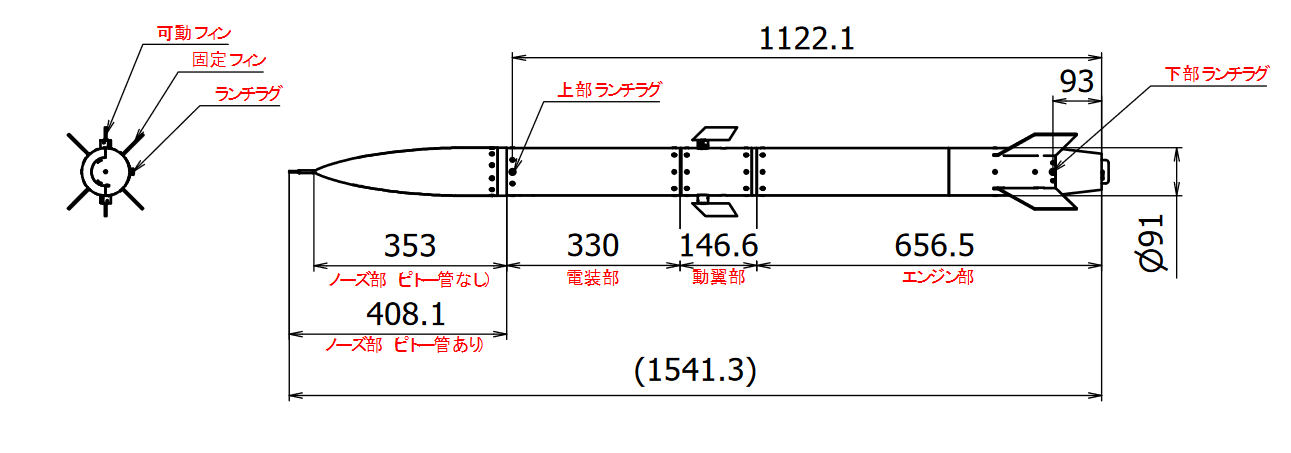
\includegraphics[scale = 0.6]{pic_str/s_sunpou.png}
    \caption{機体外形図}
    \label{s_gaikei}
\end{figure}

\begin{figure}[H]
    \centering
    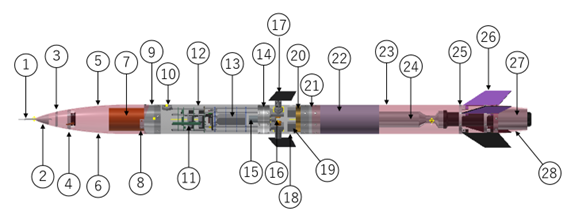
\includegraphics{pic_str/s_iti.png}
    \caption{各部材位置}
    \label{s_iti}
\end{figure}

\renewcommand{\arraystretch}{0.9}
\begin{longtable}[H]{cclll}
    \caption{各部品詳細図}
    \label{s_buhin}                                                    \\
    \toprule
    区画    & No. & 部品名       & 材質    & 型番及び説明                           \\ \hline \endhead
    ノーズ部  & 1   & ピトー管      & A5052 & 内製                               \\
          & 2   & ノーズトップ    & ABS   & ピトー管固定用                          \\
          & 3   & ピトー管用基板   & N/A   & 電装概要に記載                          \\
          & 4   & 減速機構      & N/A   & 従来機体から踏襲                         \\
          & 5   & ノーズコーン    & CFRP  &                                  \\
          & 6   & フェアリング    & CFRP  & 開放部                              \\
          & 7   & パラシュート    & ナイロン  &                                  \\
          & 8   & リカバリーネイル  & ABS   & フェアリング抑え                         \\\midrule
          & 9   & NAカプラー    & A5052 &                                  \\ \midrule
    電装部   & 10  & 電源投入スイッチ  & ABS   & \ref{switch}項に記載                 \\
          & 11  & 電装タワー     & N/A   & \ref{avi_all}章に記載                \\
          & 12  & 電装チューブ    & GFRP  &                                  \\
          & 13  & LiFeバッテリー & N/A   & ROBOパワーセル F3-1450タイプ(Li-Fe)      \\ \midrule
          & 14  & ARカプラー    & A5052 &                                  \\ \midrule
    動翼部   & 15  & 動翼制御用モータ  & N/A   & Maxon(製品番号:134164、110160、201937) \\
          & 16  & 動翼機構      & N/A   & \ref{douyoku}節に記載                \\
          & 17  & 可動フィン     & アクリル  &                                  \\
          & 18  & 動翼チューブ    & CFRP                                     \\
          & 19  & カメラ       & N/A   & MD25                             \\
          & 20  & 錘         & 真鍮    &                                  \\\midrule
          & 21  & REカプラー    & A5052 &                                  \\ \midrule
    エンジン部 & 22  & スタイロフォーム  & N/A   & エンジン抑え                           \\
          & 23  & エンジンチューブ  & CFRP                                     \\
          & 24  & エンジン      & N/A   & HyperTEK J250                    \\
          & 25  & フィンブロック   & ABS   & 固定フィン固定用                         \\
          & 26  & 固定フィン     & アクリル  &                                  \\
          & 27  & エンジン受け    & A5052 & 2部品で構成                           \\
          & 28  & テールコーン    & ABS   & \ref{tale}項に記載                   \\
    \bottomrule
\end{longtable}
\renewcommand{\arraystretch}{1.0}


\begin{figure}[H]
    \centering
    \includegraphics[scale = 0.1]{pic_str/s_59_real_pic.jpg}
    \caption{実機写真}
    \label{s_real1}
\end{figure}

\begin{figure}[H]
    \centering
    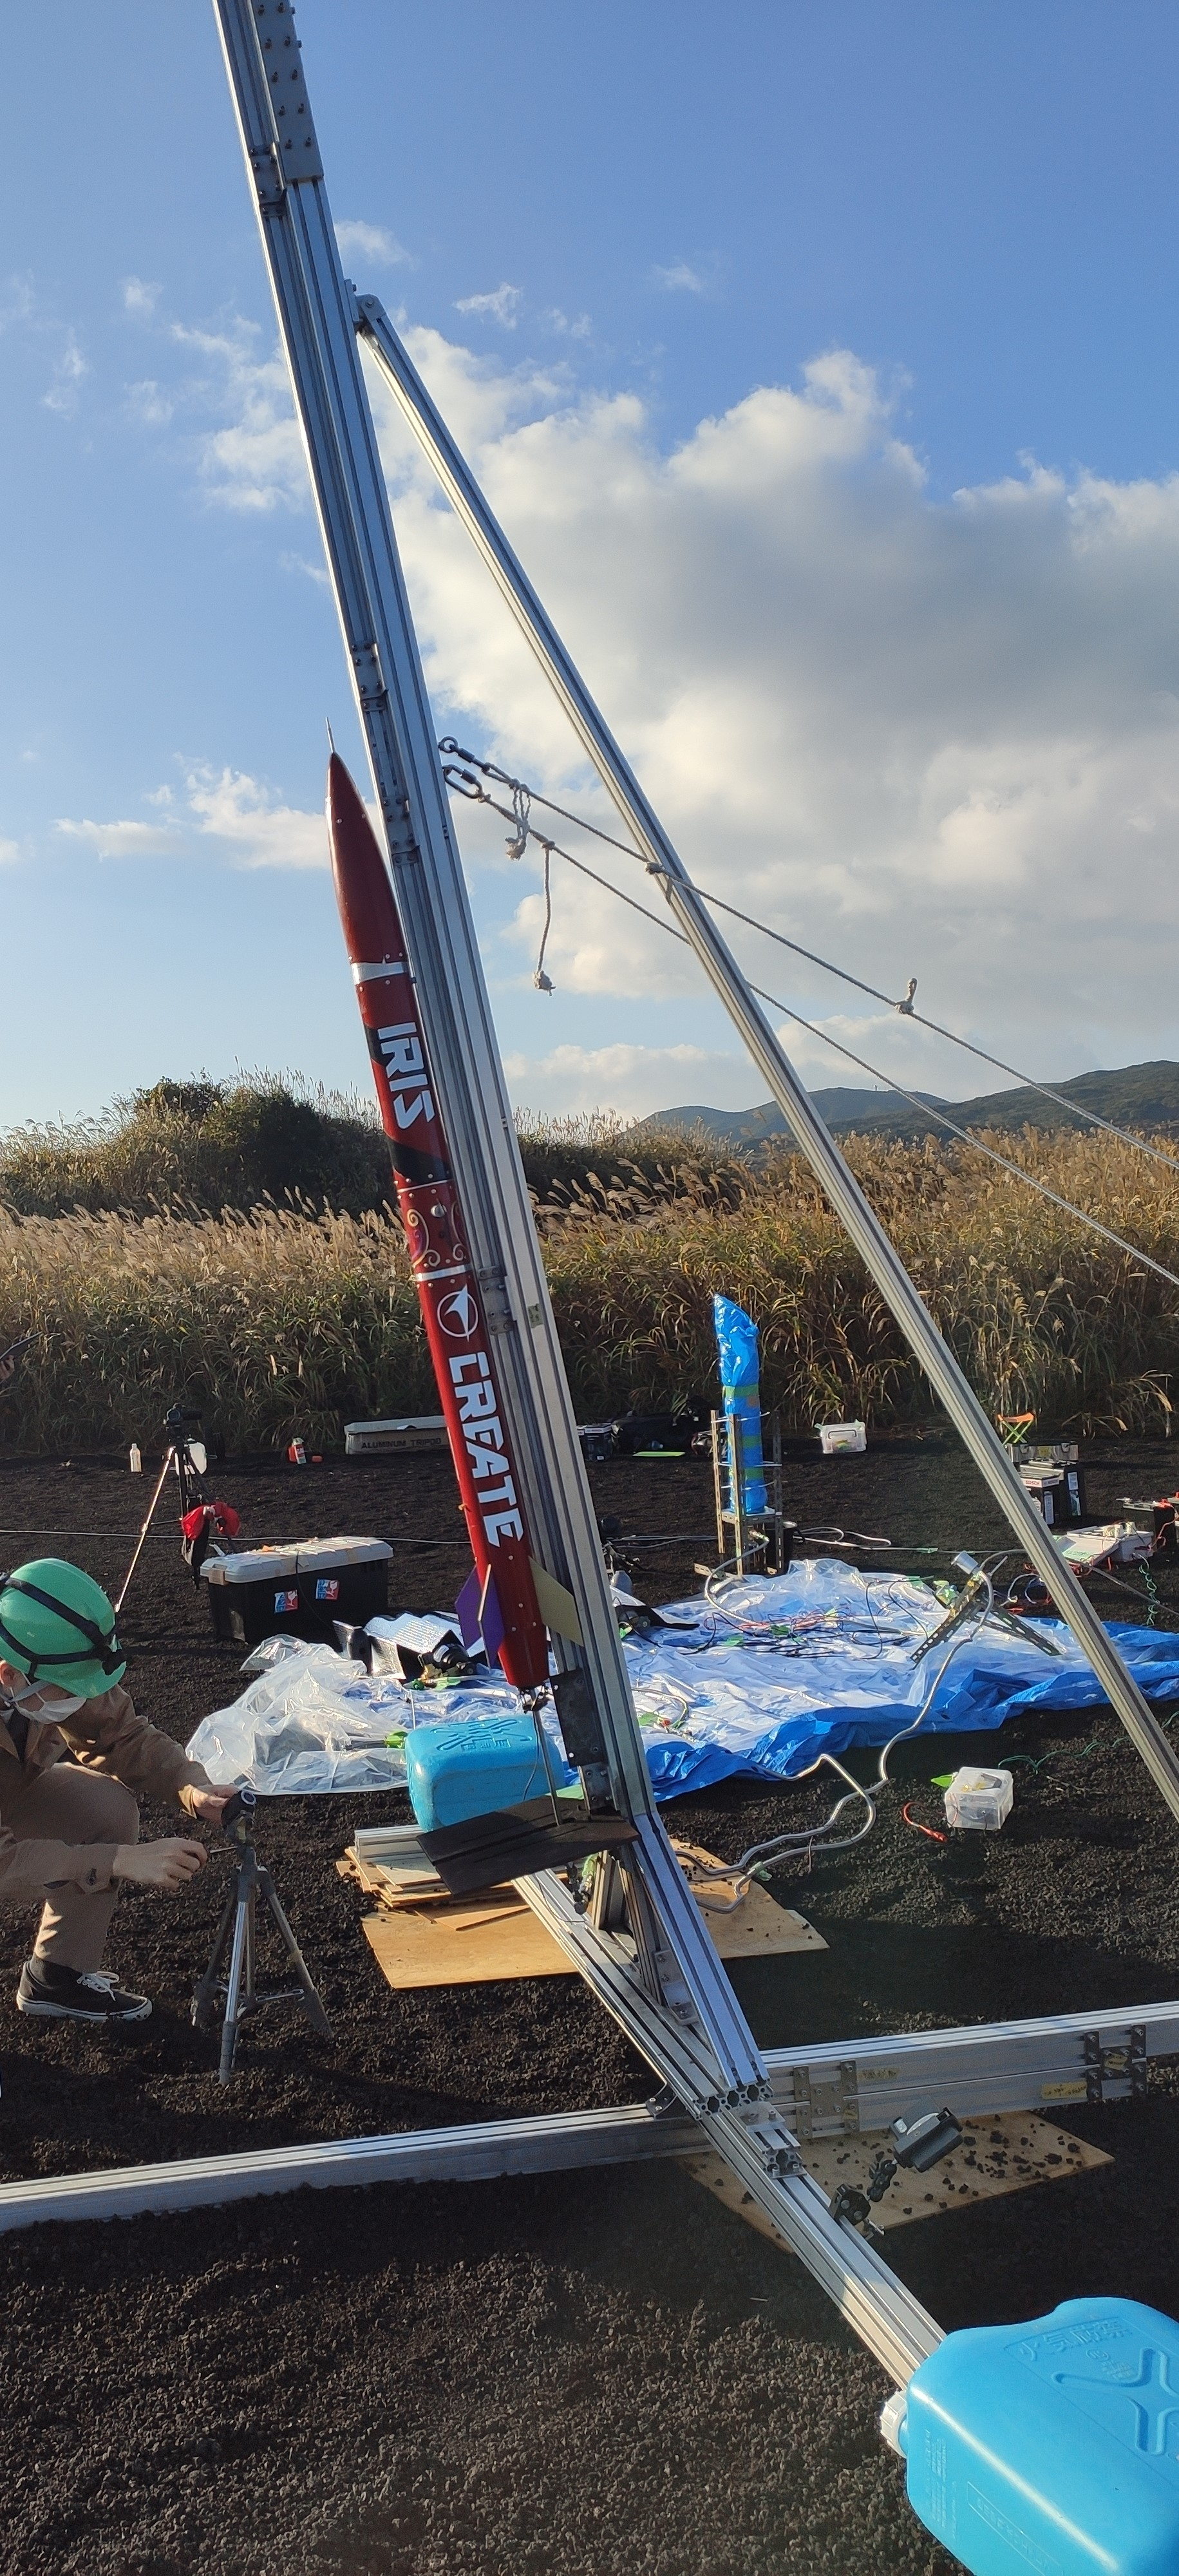
\includegraphics[scale = 0.1]{pic_str/s_59_launcher.jpg}
    \caption{実機写真(ランチャー挿入)}
    \label{s_real2}
\end{figure}

本機はロール制御ミッション達成のため、新たに可動フィンを設置していることが特徴である。
図\ref{s_gaikei}左側記載の側面図に示すように、固定フィン4枚、可動フィン2枚を搭載している。
フィンの位相角は、ランチラグを\SI{0}{deg}としたとき、固定用フィンは\SI{45}{deg}、\SI{135}{deg}、\SI{225}{deg}、\SI{315}{deg}であり、可動フィンは\SI{90}{deg}、\SI{270}{deg}となっている。
これは、可動フィンによって発生した乱流が後方の固定フィンに影響を与えないようにするためである。
また、可動フィンを取り付けない状態と取り付けた状態の両方で$F_{ST}$の基準を満たしていることをシミュレーションで確認しており、空力安定性は保たれている。

\subsection{動翼機構}
\label{douyoku}
本節では、ロール制御ミッションのために新たに追加した動翼部について記す。
動翼機構のCAD図と写真、外形の様子をそれぞれ図\ref{s_r_all}、図\ref{s_r_pic}、図\ref{s_r_outer}に示す。

\begin{figure}[H]
    \centering
    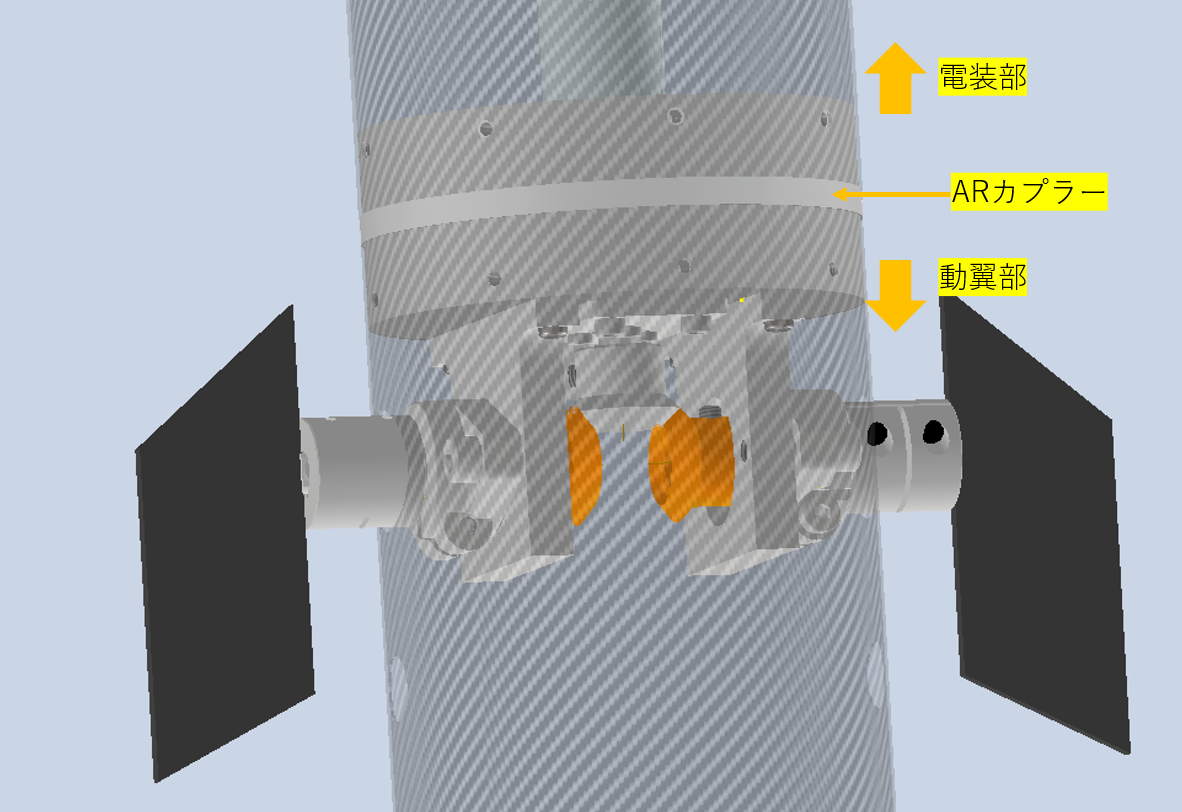
\includegraphics[scale = 0.3]{pic_str/s_roll_all.png}
    \caption{動翼機構CAD図}
    \label{s_r_all}
\end{figure}

\begin{figure}[H]
    \centering
    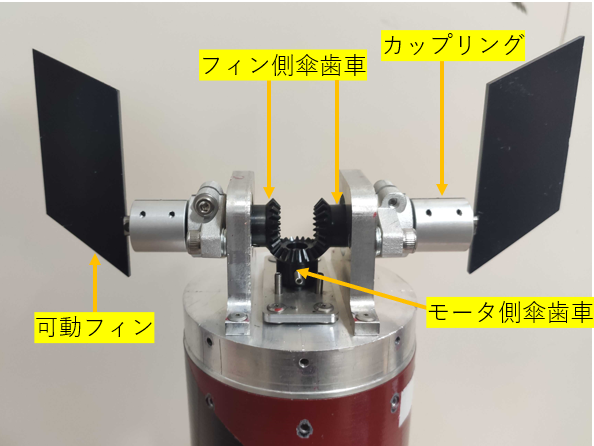
\includegraphics[scale = 0.6]{pic_str/s_r_pic.png}
    \caption{動翼機構}
    \label{s_r_pic}
\end{figure}

\begin{figure}[H]
    \centering
    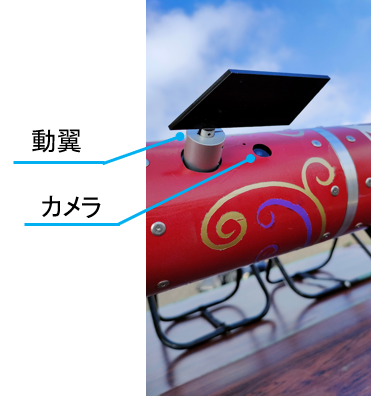
\includegraphics[scale = 0.55]{pic_str/s_r_outer.png}
    \caption{動翼部外形}
    \label{s_r_outer}
\end{figure}

傘歯車を介して、モータの回転を左右2枚の可動フィンに伝える機構になっている。
このような機構にすることで、2枚の可動フィンが連動し、かつ同じ量だけ回転するようにしている。\footnote{
    傘歯車を使用せず、左右にサーボモータを設置しフィンを回転させる方法も検討したが、高精度の制御ができるモータを使用したい、左右2つのフィン回転量が等しいことを担保したい、という2点よりこの機構を採用した。
    代わりに傘歯車のバックラッシが小さく、かつ摩擦補償が小さい機構の製作が必要となった。}

以下に特記点を示す。
\begin{itemize}
    \item フィン側傘歯車と可動フィンは連動して回転するようになっているが、左右2枚の可動フィンの位相を合わすために、カップリングを設置している。
          現地組立では水準器を使用し、2枚の可動フィンと機軸の水平度を測ることでフィン位相を合わせた。
          \\
    \item 電装計器の誤作動、電源喪失、ピトー管からの対気速度値異常などが原因で可動フィンが想定より多く回転してしまい、機体の姿勢が不安定になってしまう可能性がわずかながらある。この状況を防ぐため、フィンの回転制御角を物理的に制限する機構を搭載している。この機構のCAD図を図\ref{s_r_kadouiki}に示す。
          \begin{figure}[H]
              \centering
              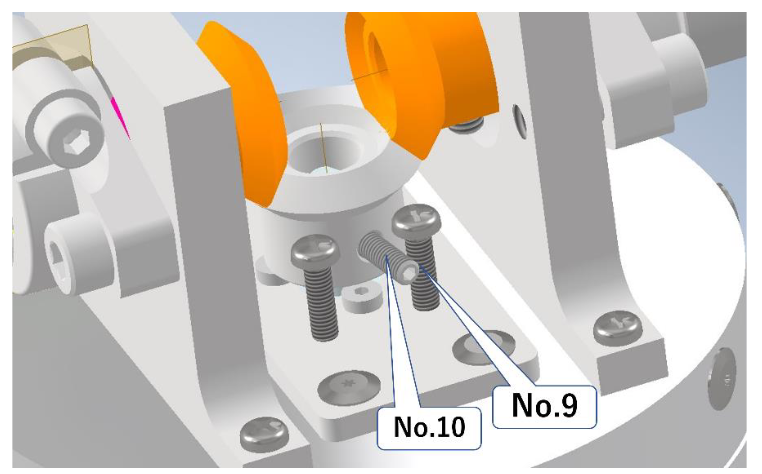
\includegraphics[scale = 0.5]{pic_str/s_r_kadouiki.png}
              \caption{回転角制御機構}
              \label{s_r_kadouiki}
          \end{figure}
          モータと傘歯車を締結しているイモネジ(No.10)を仕様より長いものを使用し、回転角が中央\footnote{2つ設置してあるネジ(No.9)から等距離の地点。}から$\pm \SI{15}{deg}$ を超えるとネジ(No.9)に当たり、止まるようになっている。
          また、制御開始時にイモネジが中央に位置していないといけないが、カップリングの印をつけることで、フィン位相をあわせる際にイモネジが中央位置かどうかを分かるようにした。
          また、イモネジの正しい使い方をしていないため、通常使用時から緩むようになっていたが、ネジロックを使用することで緩まないようにした。
          \\
    \item 前述の通り、バックラッシを調整できるような設計を行った。主に加工誤差が原因で、傘歯車を設計値通りの場所に設置することができないため、製作後に傘歯車の位置をワッシャーとシムリングを挟むことでで調整できるようにした。
          実際に\SI{0.1}{mm}ごとに傘歯車の位置を調整していき、バックラッシが小さくなり、かつ摩擦補償が小さくなる位置を決定した。
          \\
    \item 図\ref{s_r_outer}に示すように、動翼のすぐ下にカメラを設置した。これは飛行中に動翼が正常に動作していることを確認するため、及びロールしない映像を撮影するためである。
\end{itemize}


\newpage
\subsection{テールコーン}
\label{tale}

\red{ロケットの乱流を~~}のため、機体後端にテールコーンを設置した。
テールコーン付近の断面図を図\ref{s_tale_num}に、主な構成部品を表\ref{s_tale_table}に示す。
また、テールコーンの図面を図\ref{s_tale_zumen}に示す。
テールコーンを使用した際の効果についてはシミュレーション系の章で記す。

\begin{figure}[H]
    \centering
    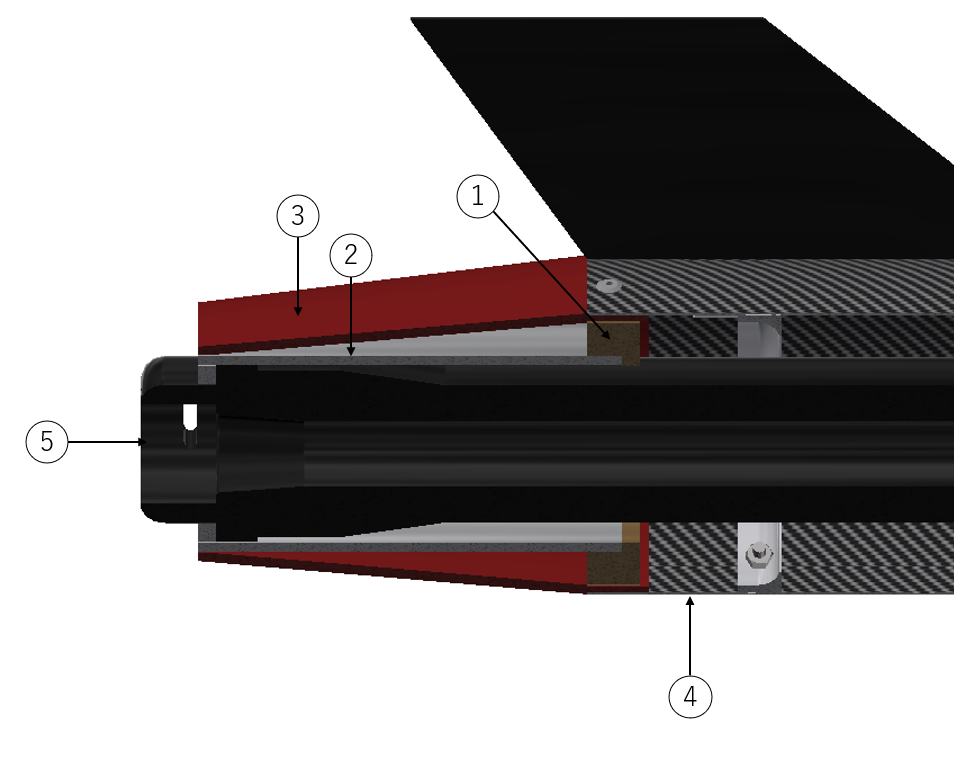
\includegraphics[scale = 0.4]{pic_str/s_talecorn_num.png}
    \caption{テールコーン付近断面図}
    \label{s_tale_num}
\end{figure}

\begin{table}[H]
    \centering
    \caption{テールコーン部品表}
    \begin{tabular}{ccc} \toprule
        No. & 名称       & 材質、型番         \\ \midrule
        1   & エンジン受け1  & A5052         \\
        2   & エンジン受け2  & A5052         \\
        3   & テールコーン   & ABS           \\
        4   & エンジンチューブ & CFRP          \\
        5   & エンジン     & HyperTEK J250 \\ \bottomrule
    \end{tabular}
    \label{s_tale_table}
\end{table}

\begin{figure}[H]
    \centering
    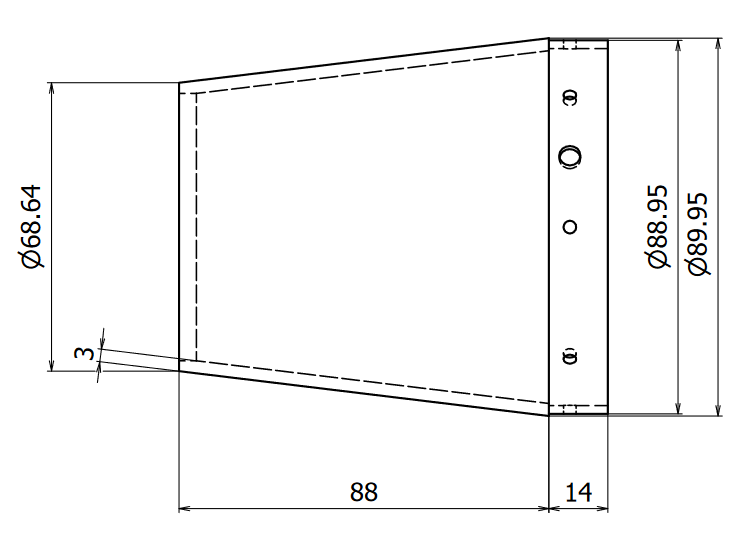
\includegraphics[scale = 0.6]{pic_str/s_talecorn_zumen.png}
    \caption{テールコーン図面}
    \label{s_tale_zumen}
\end{figure}

\vspace{30mm}

\section{打上結果(構造関係)}
\begin{comment}
\subsection{機体組立}
本打上実験ではウィンドウの順番が事前に決められておらず、現地審査合格状況とGSE展開状況で順番が決める事になっていたため、現地ではできるだけ短時間で組立られるような工夫をした。
具体的にはエンジン部はフィン含め完全に組み立てる、電装タワーも組み立てて行き当日一部配線のみを繋ぐ、組立練習を複数回行う等を行った。

打上実験1日目は、8:10頃打上実験本部に到着後すぐ組立を開始し、予定より10分ほど遅れて9:00頃に機体が完成した。
その後現地審査担当の到着と他機体の現地審査を待ち、9:45頃に本機体の現地審査を開始した。
現地審査では、完成報告書と最終審査書に不備があることが発覚した。
しかし、その場でシミュレーションを行った上で問題が無いことを確認し、10:45頃に現地審査の合格した。
その後、11:40頃本部から射点に向けて機体を搬入した。
CRETAE1が13:00X、CREATE2(本機)が14:00Xの予定であったが、CREATE1打上げの際のGSEトラブルの影響で実験1日目の打上げは断念し、翌日に打ち上げることとした。

打上実験2日目は、午前2:20宿出発、2:40裏砂漠駐車場着、3:10裏砂漠駐車場発、3:45本部到着、というスケジュールで動き、風と気温の様子を見て4:20頃に組立を開始した。
2日目はおおよそ順調に進み、5:20には現地審査合格、6:00には射点に機体搬入完了した。
7:20頃からランチャー挿入、ステム挿入、ランチャー立上げ、総員退避が行われ、7:47に打上げられた。

\end{comment}


\subsection{機体回収}
打上げは正常に点火し、離床後10.2秒後に減速機構が作動し、正常にパラシュートが開傘した。

着地状況を図\ref{s_tyakuti_pic}に示す。
\begin{figure}[H]
    \centering
    \includegraphics[scale = 0.08]{pic_str/s_tyakuti_pic.jpg}
    \caption{着地状況}
    \label{s_tyakuti_pic}
\end{figure}

落下の衝撃でアクリル製の固定フィンと可動フィンが機体から外れ、機体の周りに散らばっている様子が確認できた。
また、CFRP製のノーズコーンも落下の衝撃で割れていることが確認でき、チューブの塗装が一部めくれ傷がついていた。
しかし、それ以外の搭載計器やエンジン、動翼機構には問題無いことをその後確認した。


\end{document}